% ============================================================
%  Chapter 6 — In Practice
% ============================================================
\chapter{In Practice}
\label{ch:practice}

The previous chapter measured the decomposition; this chapter puts it to use.
Separating a photograph into an illuminant-invariant albedo and a coloured shading
layer is not only an estimation target but a practical handle: once the two factors
are available, an image can be altered by changing one of them and leaving the other
untouched, which no edit on the entangled pixels can do. This chapter develops that
idea into a single application, \emph{factor-space editing}, and presents two instances
of it that follow directly from the properties established in \chapref{ch:experiments}.

This chapter is a proof of concept, not a second evaluation. Each edit is defined
directly on the predicted factors, and its behaviour follows from how those factors are
constructed, so the argument is made by formulation rather than by a quantitative
application study, for which no user study or application-specific metric is available.
Every factor comes from the single trained model selected in \secref{sec:arap_results},
labelled simply \emph{Ours}; the chapter draws no comparison between internal
checkpoints. That model's decomposition is shown first (\figref{fig:decomposition}), and
the two edits are then read as operations on its predicted albedo, shading, and residual.

All edits below start from the decomposition
$\mathbf{I} = \mathbf{A}_d \odot \mathbf{S}_d + \mathbf{R}$,
where $\mathbf{A}_d$ is the predicted diffuse albedo, $\mathbf{S}_d$ the coloured diffuse
shading, and $\mathbf{R} = (\mathbf{I} - \mathbf{A}_d \odot \mathbf{S}_d)_{+}$ the
analytic non-diffuse residual that captures specular highlights, visible light
sources, and clipped regions (\secref{sec:physics}).

\begin{figure}[H]
  \centering
  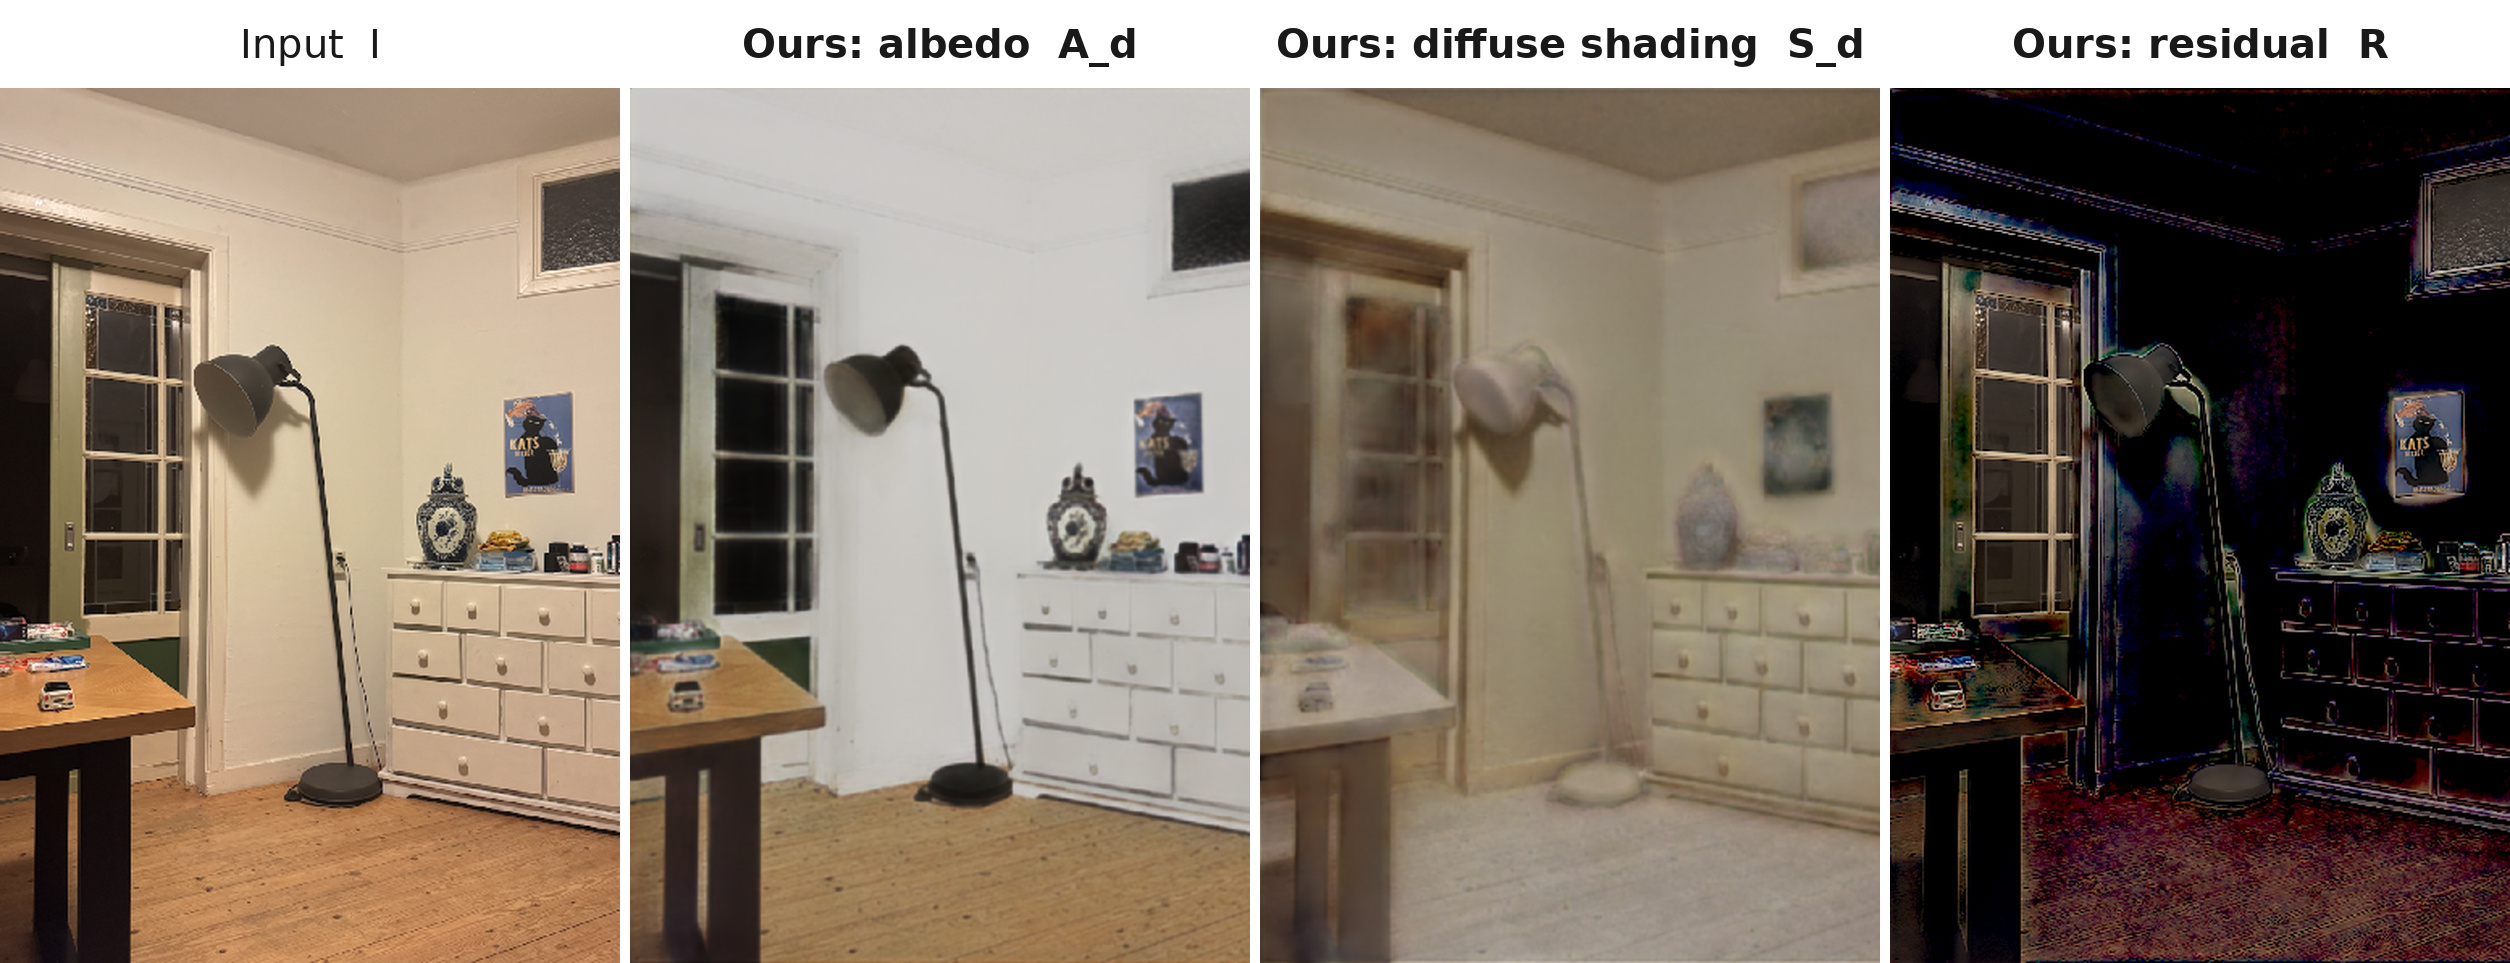
\includegraphics[width=\textwidth]{images/ch6/decomposition.jpg}
  \caption[Predicted decomposition of a realistic indoor photograph.]{%
    Predicted decomposition by Ours on a realistic indoor photograph. From
    left: input photograph; predicted diffuse albedo $\mathbf{A}_d$; diffuse shading
    $\mathbf{S}_d=(1-\boldsymbol{\pi})/\boldsymbol{\pi}$ obtained by inverting
    the model's inverse-domain shading output $\boldsymbol{\pi}$; and the analytic residual
    $\mathbf{R}=(\mathbf{I}-\mathbf{A}_d\odot\mathbf{S}_d)_{+}$. Albedo and
    shading are independently normalised for display. The residual is shown at
    its calculated magnitude, without amplification, so it remains dark except
    at bright non-diffuse regions such as glass and highlights. This is a
    qualitative factorisation, not ground truth. The four panels are direct
    crops from the saved visualization; no new inference or post-hoc colour
    correction is applied for this figure.
  }
  \label{fig:decomposition}
\end{figure}

We do not include a cross-illuminant transfer demonstration, in which one scene is
re-rendered under another scene's illuminant. Its natural score, the PSNR of the
recomposed image, is highest for the visibly desaturated colour-path-off ablation,
because compensating albedo and shading errors cancel in their product; it is a
gameable factor-consistency diagnostic rather than evidence of physical correctness.
The two edits below instead each act on a single factor of the decomposition, one on the
residual $\mathbf{R}$ and one on the shading $\mathbf{S}_d$, so their behaviour follows
directly from how those factors are defined.


\section{Factor-Space Editing}
\label{sec:factor_edit}

\paragraph{Residual-space suppression}

The residual layer contains image energy not represented by the predicted diffuse
product. This can include specular highlights and clipped sources, but it can also
include ordinary scene structure that the estimated albedo and shading fail to
reconstruct.
Scaling it yields the edit
\begin{equation}
  \mathbf{I}'_{\alpha}
  \;=\;
  \mathbf{A}_d \odot \mathbf{S}_d + \alpha\,\mathbf{R},
  \qquad \alpha \in [0, 1] .
  \label{eq:glare}
\end{equation}
Setting $\alpha < 1$ dims energy assigned to the residual while holding the
model's predicted diffuse product fixed; $\alpha = 0$ removes that component
entirely.
The same operation performed in image space (for example, lowering the exposure
of bright regions) also changes diffuse regions; residual scaling instead holds
the model's predicted diffuse product fixed.
This is the same operation used for highlight editing by
\mycitetext{careaga24cdiid}, but whether it behaves as a selective highlight
control depends on the quality of the decomposition.

Because $\mathbf{R}$ is the analytic leftover of \figref{fig:decomposition} rather than a
segmented highlight region, reducing $\alpha$ suppresses everything the diffuse product
fails to explain, diffuse surfaces included, not one isolated highlight. Residual scaling
is therefore a targeted edit on a predicted factor, not a semantic glare mask or a
general-purpose glare remover; how selective it appears is governed entirely by the
quality of the decomposition.

\paragraph{Illumination editing}

Classic brightness or contrast adjustments operate on the entangled image, so
lifting dark regions also washes out material texture and colour.
With the decomposition, tonal edits can be applied to the shading layer alone:
\begin{equation}
  \mathbf{I}'_{f}
  \;=\;
  \mathbf{A}_d \odot f(\mathbf{S}_d) + \mathbf{R},
  \label{eq:illum_edit}
\end{equation}
where $f$ is a monotone luminance gain. Because our shading is unbounded, we do
not apply $\mathbf{S}_d^{\gamma}$ directly. We normalise shading luminance by its
95th percentile $q_{95}$ and use
\begin{equation}
 f_{\gamma}(\mathbf{S}_d)
 = \mathbf{S}_d
 \left[\operatorname{clip}\!\left(
 \frac{L(\mathbf{S}_d)}{q_{95}},\varepsilon,1\right)\right]^{\gamma-1},
 \qquad 0<\gamma<1 ,
 \label{eq:shadow_lift}
\end{equation}
with the gain capped at $2.5$. Low predicted illumination is lifted while values
at or above the reference percentile are unchanged.
Because $\mathbf{A}_d$ is untouched, the model's predicted material colours and
texture are held fixed while its predicted illumination changes.
This is where the invariance targeted throughout the thesis pays off directly: an
albedo that does not carry the illuminant's colour can be re-lit without its materials
drifting in hue, so lifting a dark, warm-lit corner reveals the surfaces' own colour
rather than amplifying the lamp's cast. The result is a shading edit built directly on
the decomposition, and its fidelity is bounded by how completely that cast was removed
in the first place.

By construction this holds the predicted albedo of \figref{fig:decomposition} fixed,
whereas the same luminance gain applied to the entangled image multiplies material and
illumination together and so shifts material appearance as well. The edit is therefore a
statement about controllability of the predicted factors, not about ground-truth
preservation.

Both edits succeed exactly to the degree the decomposition does, and their two
failure modes map onto the two axes measured in \chapref{ch:experiments}. Wherever
some illuminant colour has leaked into the albedo (the residual cast quantified by the
MID and ARAP constancy metrics), that component is already baked into the material
layer and will not respond to a shading edit. And wherever the shading is structurally
soft (a sharp shadow boundary that was never fully separated from the albedo), scaling
the shading cannot cleanly remove it. Neither limitation is repaired by the editing
operation; each is inherited from the factors being edited, which is why the constancy
and structure results of the previous chapter are what ultimately bound how far this
application can be taken.
